\documentclass[conference]{IEEEtran}
\IEEEoverridecommandlockouts

\usepackage[utf8]{inputenc}
\usepackage[T1]{fontenc}
\usepackage{lmodern}
\usepackage{amsmath,amssymb}
\usepackage{graphicx}
\usepackage{booktabs}
\usepackage{multirow}
\usepackage{array}
\usepackage{xcolor}
\usepackage{tikz}
\usetikzlibrary{arrows.meta,positioning,fit,shapes.geometric}
\usepackage{pgfplots}
\pgfplotsset{compat=1.17}
\usepackage[hidelinks]{hyperref}
\usepackage{url}
\usepackage{cite}

% Placeholder macro: shows missing details in red until they are filled in.
\newcommand{\placeholder}[1]{\textcolor{red}{[#1]}}

\begin{document}

\title{MicroRCA-Agent: Toward Evidence-Grounded Agentic Root Cause Analysis for Microservice Systems\\
\large Project Code: G2-07}

\author{
\IEEEauthorblockN{Ibrahim Umar Malik}
\IEEEauthorblockA{Roll No.\ 22I-2315\\
FAST-NUCES, Islamabad\\
\texttt{i222315@nu.edu.pk}}
\and
\IEEEauthorblockN{Syed Mustafa Ali}
\IEEEauthorblockA{Roll No.\ 22I-2304\\
FAST-NUCES, Islamabad\\
\texttt{i222304@nu.edu.pk}}
\and
\IEEEauthorblockN{Fasih Shahid Abbasi}
\IEEEauthorblockA{Roll No.\ 22I-2235\\
FAST-NUCES, Islamabad\\
\texttt{i222235@nu.edu.pk}}
\and
\IEEEauthorblockN{Hamza Ijaz}
\IEEEauthorblockA{Roll No.\ 22I-2330\\
FAST-NUCES, Islamabad\\
\texttt{i222330@nu.edu.pk}}
}

\maketitle

% =====================================================================
\begin{abstract}
When a microservice system fails, the user-visible symptom frequently surfaces in a service other than the one that initiated the fault, and operators must reconcile metrics, logs, traces, and call-graph structure to localize the cause. Recent studies apply tool-using large language model (LLM) agents to this task, but report low accuracy, unverified hypotheses, and unbounded investigation cost. This paper presents MicroRCA-Agent, an evaluation-ready framework for agentic root cause analysis (RCA). It contributes typed incident and diagnosis contracts with label blinding, six bounded observability tools, provider-agnostic LLM adapters, statistical and single-call baselines, a ReAct-style investigator with step and tool budgets, and a shared harness that records accuracy together with model calls, tool calls, tokens, and latency. On 101 labelled failures from the Online Boutique and Train-Ticket systems in the Nezha benchmark, reciprocal-rank fusion of metric, log, and trace evidence raises top-1 localization accuracy (AC@1) from 0.178 to 0.307 relative to metrics-only scoring (McNemar exact $p=0.001$), at a mean cost of 0.009\,s per case. A leave-one-signal-out ablation shows that most of this gain is attributable to fusing CPU and memory evidence rather than to logs or traces. A failure analysis of the fused baseline finds that 25 of its 70 top-1 errors rank a direct caller or callee of the true root cause first, and that accuracy collapses on Train-Ticket (AC@1 0.156) and on code-level faults (AC@1 $\le$0.111). These results quantify where statistical scoring fails and motivate the verification, cost-control, and memory mechanisms of the proposed agent. Accuracy results for the LLM-based methods are not yet available and are not claimed.
\end{abstract}

\begin{IEEEkeywords}
microservices, root cause analysis, agentic AI, large language models, observability, ReAct, AIOps
\end{IEEEkeywords}

% =====================================================================
\section{Introduction}

Microservice architectures decompose an application into independently deployed services that communicate over the network~\cite{dragoni2017microservices}. A single user request may traverse many such services, so a fault in one component commonly manifests as elevated latency or errors in its callers. The resulting gap between \emph{where a failure is observed} and \emph{where it originates} makes root cause analysis (RCA) one of the most time-consuming activities in incident response~\cite{soldani2022survey,zhou2021trainticket}. Operators must correlate resource metrics, application logs, and distributed traces, and must reason over the service dependency graph to separate causes from downstream symptoms.

Two families of automated RCA have emerged. Statistical and graph-based methods score services by anomaly magnitude, causal structure, or trace spectra~\cite{wu2020microrca,wang2018cloudranger,meng2020microcause,yu2021microrank,li2021tracerca,li2022circa,pham2024baro}. They are fast and reproducible, but their scoring rules are fixed and they rarely explain their conclusions. More recently, LLM-based systems have been proposed that reason over incident data and invoke tools~\cite{ahmed2023recommending,chen2024rcacopilot,wang2024rcagent,roy2024exploring}. The OpenRCA benchmark, which we adopt as our base paper, evaluates such agents on 335 failures from three enterprise systems and reports that even the best configuration, an RCA-agent driven by Claude~3.5, solved only 11.34\% of failure cases~\cite{xu2025openrca}.

\textbf{Research gaps.} From the Phase~1 literature review we identify four gaps that motivate this work. \emph{G1 (verification):} agentic RCA systems typically accept the first plausible hypothesis, without checking whether the implicated service is a cause or a propagated symptom~\cite{xu2025openrca,roy2024exploring}. \emph{G2 (cost awareness):} published agents seldom bound or report the number of model calls, tool calls, and tokens consumed per incident, which obscures whether accuracy gains justify their cost~\cite{chen2023frugalgpt}. \emph{G3 (incident memory):} each incident is investigated from scratch, even though recurring fault patterns are common in production~\cite{chen2024rcacopilot}. \emph{G4 (multimodal grounding):} many methods rely on a single telemetry modality, whereas faults such as exceptions or wrong return values may be visible only in logs or traces~\cite{yu2023nezha,lee2023eadro}.

\textbf{Research questions.} This paper addresses the following questions.
\begin{itemize}
\item \textbf{RQ1 (G4).} Does fusing metric, log, and trace evidence improve service-level localization over metrics-only scoring, and which signals contribute to the improvement?
\item \textbf{RQ2 (G1).} To what extent are localization errors explained by fault propagation along the call graph, which a verification step would target?
\item \textbf{RQ3 (G2).} What are the per-incident costs of the evaluated methods, and can agentic investigation be bounded and accounted for in the same harness?
\item \textbf{RQ4 (G1--G3).} Does a tool-using agent with verification, budget control, and memory outperform statistical and single-call baselines at acceptable cost? We state RQ4 as a hypothesis with an evaluation protocol; it is not answered in this paper.
\end{itemize}

\textbf{Contributions.} The contributions of this work are:
\begin{enumerate}
\item A reproducible RCA framework with typed contracts, label blinding, compact multimodal incident bundles, and six JSON-schema observability tools shared by all methods~\cite{g207microrcaagent}.
\item A family of comparable methods, namely two statistical baselines (B0), a single-call LLM baseline (B1), and a budgeted ReAct-style investigator (P0) with interfaces for verification and memory, evaluated by one harness that records quality and cost.
\item An empirical characterization of statistical RCA on 101 Nezha incidents, including significance testing, a signal ablation, and a categorized failure analysis that quantifies the symptom-propagation errors targeted by G1.
\end{enumerate}

% =====================================================================
\section{Related Work}

\textbf{Statistical and graph-based RCA.} Early microservice RCA methods construct a dependency or anomaly graph and rank services with random walks or PageRank-style propagation. CloudRanger builds an impact graph from metrics using causal discovery~\cite{wang2018cloudranger}; MicroRCA attributes anomalies on an attributed service graph~\cite{wu2020microrca}; and MicroCause combines causal inference with temporal propagation to localize failures among metrics~\cite{meng2020microcause}. CIRCA formulates RCA as intervention recognition on a causal Bayesian network~\cite{li2022circa}, while BARO detects multivariate change points and ranks root causes robustly~\cite{pham2024baro}. Trace-centric methods such as MicroRank~\cite{yu2021microrank} and TraceRCA~\cite{li2021tracerca} exploit span structure and spectrum analysis, and Groot constructs event graphs for industrial-scale RCA~\cite{wang2021groot}. Survey work catalogues these approaches and notes their reliance on hand-crafted scoring rules and single data sources~\cite{soldani2022survey}.

\textbf{Multimodal RCA.} Nezha mines interpretable patterns across metrics, logs, and traces and localizes root causes at code and resource granularity; it also released the fault-injection dataset used in this study~\cite{yu2023nezha}. Eadro jointly learns anomaly detection and localization from multi-source data~\cite{lee2023eadro}. Benchmarks such as RCAEval~\cite{pham2025rcaeval}, together with the Train-Ticket~\cite{zhou2021trainticket}, DeathStarBench~\cite{gan2019deathstarbench}, and Online Boutique~\cite{google2024onlineboutique} systems, enable reproducible comparison. Our statistical baselines borrow the robust-deviation scoring used by such detectors~\cite{leys2013mad} and fuse modalities with reciprocal-rank fusion~\cite{cormack2009rrf}.

\textbf{LLMs and agents for incident management.} Ahmed et al.\ showed that fine-tuned LLMs can recommend root causes and mitigations for cloud incidents~\cite{ahmed2023recommending}. RCACopilot retrieves historical incidents and diagnostic outputs to predict root-cause categories~\cite{chen2024rcacopilot}, and RCAgent equips an autonomous agent with tools over cloud data~\cite{wang2024rcagent}. Roy et al.\ evaluated ReAct agents on production incidents and reported both promise and failure modes such as hallucinated evidence~\cite{roy2024exploring}. These systems build on general agent techniques: chain-of-thought prompting~\cite{wei2022cot}, interleaved reasoning and acting (ReAct)~\cite{yao2023react}, tool use~\cite{schick2023toolformer}, self-consistency~\cite{wang2023selfconsistency}, iterative self-feedback~\cite{madaan2023selfrefine,shinn2023reflexion}, and memory-augmented agents~\cite{park2023generative}; a broader survey is given in~\cite{wang2024agentsurvey}. Cost-aware LLM usage has been studied in FrugalGPT~\cite{chen2023frugalgpt}, but it is rarely reported in RCA evaluations.

\textbf{Positioning against the base paper.} OpenRCA~\cite{xu2025openrca} defines RCA as identifying the originating component, time, and reason of a failure from raw telemetry, and provides an RCA-agent that writes and executes analysis code. Its low solve rate establishes that unconstrained agentic RCA remains difficult. MicroRCA-Agent differs in three respects. First, it exposes a small set of typed, bounded tools rather than open-ended code execution, which constrains the action space and makes tool usage auditable. Second, it evaluates every method, statistical or agentic, through one harness that records cost alongside accuracy (G2). Third, it reserves explicit interfaces for hypothesis verification (G1) and incident memory (G3), which OpenRCA's agent does not provide. Because OpenRCA uses different systems, labels, and a stricter success criterion, its numbers are not directly comparable with ours (Section~\ref{sec:evalmethod}).

% =====================================================================
\section{Problem Formulation}\label{sec:problem}

Let a microservice system have a service set $S=\{s_1,\dots,s_n\}$ and a directed call graph $G=(S,E)$, where $(s_i,s_j)\in E$ indicates that $s_i$ calls $s_j$. An \emph{incident} $c$ is reported at alert time $t_a$ and is associated with telemetry $\mathcal{T}_c=(M_c,L_c,R_c)$: per-service metric series $M_c$, log statistics $L_c$, and trace statistics $R_c$, each covering a pre-alert reference window and a post-alert window. Each incident carries a ground-truth label $y_c=(s^\ast_c,f^\ast_c)$, where $s^\ast_c\in S$ is the root-cause service and $f^\ast_c\in F$ is a fault type from the set $F=\{$\texttt{cpu\_contention}, \texttt{cpu\_consumed}, \texttt{network\_delay}, \texttt{exception}, \texttt{return}$\}$.

\textbf{Input.} A method receives the \emph{blinded} incident $\tilde{c}=(\text{id}, \text{system}, t_a, S, E)$ with $y_c$ removed, and may query $\mathcal{T}_c$ only through the tool interface.

\textbf{Output.} A method returns a diagnosis $D_c=\langle (s_{(1)},f_{(1)},p_{(1)},e_{(1)}),\dots,(s_{(k)},f_{(k)},p_{(k)},e_{(k)})\rangle$, an ordered list of candidate services with a predicted fault type, a confidence $p\in[0,1]$, and textual evidence $e$, together with a summary. The task is service-level localization: rank $s^\ast_c$ as high as possible, and predict $f^\ast_c$ for the top candidate.

\textbf{Cost.} For each incident the harness records $u_c=(\#\text{LLM calls}, \#\text{tool calls}, \#\text{tokens}, \text{latency})$.

\textbf{Hypotheses.} Corresponding to RQ1--RQ4 we test or specify: \emph{H1}, multimodal fusion improves AC@1 over metrics-only scoring; \emph{H2}, a substantial fraction of top-1 errors place a call-graph neighbour of $s^\ast_c$ first; \emph{H3}, the investigator's cost can be bounded by step and tool budgets and recorded per incident; and \emph{H4}, the full agent improves AC@1 over B0 and B1 at a reported cost. H1 and H2 are tested in Section~\ref{sec:results}; H3 is verified at the pipeline level; H4 remains open.

% =====================================================================
\section{Proposed System}\label{sec:system}

Fig.~\ref{fig:arch} shows the architecture of MicroRCA-Agent. All methods read from the same case store and return the same diagnosis contract to the evaluation harness, which guarantees that differences in results stem from the methods rather than from data handling.

\begin{figure*}[t]
\centering
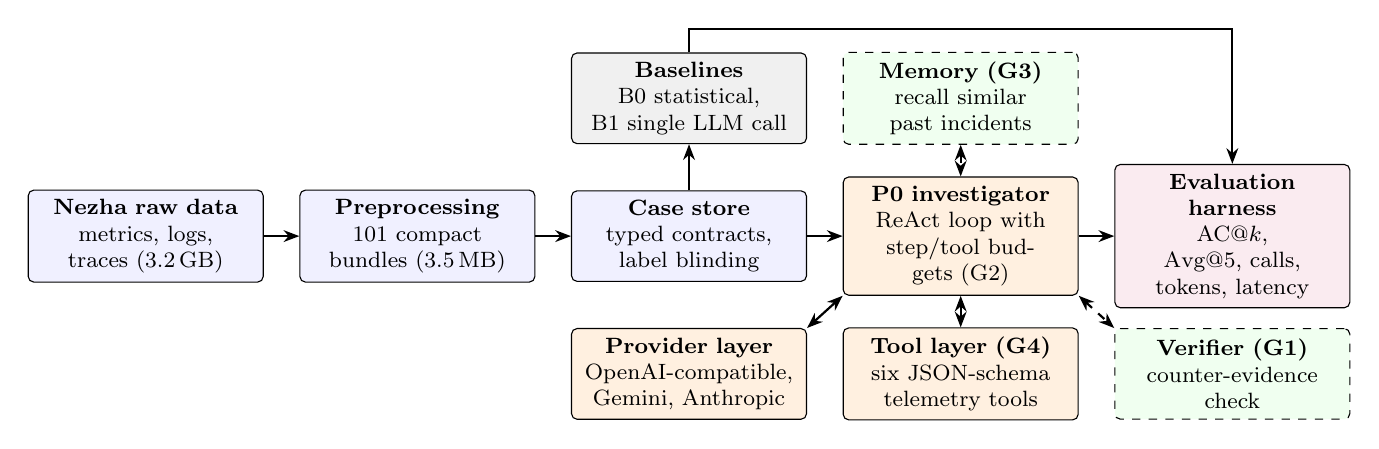
\begin{tikzpicture}[
  box/.style={draw, rounded corners=2pt, align=center, font=\footnotesize, minimum height=1.15cm, text width=2.75cm, fill=white},
  data/.style={box, fill=blue!6},
  agent/.style={box, fill=orange!12},
  base/.style={box, fill=gray!12},
  hook/.style={box, dashed, fill=green!6},
  arr/.style={-{Stealth[length=2mm]}, thick},
  darr/.style={{Stealth[length=2mm]}-{Stealth[length=2mm]}, thick}
]
\node[data]  (raw)   at (0,0)     {\textbf{Nezha raw data}\\metrics, logs,\\traces (3.2\,GB)};
\node[data]  (pre)   at (3.45,0)  {\textbf{Preprocessing}\\101 compact\\bundles (3.5\,MB)};
\node[data]  (store) at (6.9,0)   {\textbf{Case store}\\typed contracts,\\label blinding};
\node[agent] (agent) at (10.35,0)  {\textbf{P0 investigator}\\ReAct loop with\\step/tool budgets (G2)};
\node[box, fill=purple!8] (eval) at (13.8,0) {\textbf{Evaluation harness}\\AC@$k$, Avg@5, calls,\\tokens, latency};
\node[base]  (b0)    at (6.9,1.75) {\textbf{Baselines}\\B0 statistical,\\B1 single LLM call};
\node[hook]  (mem)   at (10.35,1.75) {\textbf{Memory (G3)}\\recall similar\\past incidents};
\node[agent] (prov)  at (6.9,-1.75) {\textbf{Provider layer}\\OpenAI-compatible,\\Gemini, Anthropic};
\node[agent] (tools) at (10.35,-1.75) {\textbf{Tool layer (G4)}\\six JSON-schema\\telemetry tools};
\node[hook]  (ver)   at (13.8,-1.75) {\textbf{Verifier (G1)}\\counter-evidence\\check};
\draw[arr] (raw) -- (pre);
\draw[arr] (pre) -- (store);
\draw[arr] (store) -- (agent);
\draw[arr] (agent) -- (eval);
\draw[arr] (store) -- (b0);
\draw[arr] (b0.north) -- ++(0,0.3) -| (eval.north);
\draw[darr, dashed] (mem) -- (agent);
\draw[darr] (agent) -- (tools);
\draw[darr] (prov.north east) -- (agent.south west);
\draw[darr, dashed] (agent.south east) -- (ver.north west);
\end{tikzpicture}
\caption{Architecture of MicroRCA-Agent. The case store passes only label-blinded incidents to every method, and all methods return the same diagnosis contract to the evaluation harness. Solid boxes are implemented in Phase~1; dashed boxes are interfaces whose policies (verification for G1, memory for G3) are planned for Phase~2. Budget control (G2) is enforced inside the investigator loop.}
\label{fig:arch}
\end{figure*}

\subsection{Data pipeline and contracts}
A preprocessing script converts the raw Nezha data into one compressed JSON bundle per labelled incident. Each bundle retains per-service metric series from 30\,min before to 5\,min after the alert; per-service log volume, error-like line rate, and log templates absent from fault-free logs; per-service span rate and p50/p90 span latency for both the fault window and fault-free traffic; the call graph; and the label. Log templates are obtained with a lightweight masking of identifiers and numbers, a simplified form of template mining~\cite{he2017drain}. The loader validates each bundle against Pydantic contracts (\texttt{IncidentCase}, \texttt{Diagnosis}, \texttt{RankedCause}, \texttt{AgentState}, \texttt{Usage}, \texttt{EvalRecord}); fault types are a closed enumeration and confidences are constrained to $[0,1]$. A \texttt{blind()} operation returns a copy of the incident without its label, and only this copy is passed to a method.

\subsection{Telemetry tools}
Table~\ref{tab:tools} lists the six tools. Each reads only the current incident's telemetry, returns a small JSON object that fits in an LLM context, and is described by a JSON schema compatible with OpenAI- and Anthropic-style function calling. The same functions serve all methods: B0 calls the scoring functions directly, B1 receives their outputs precomputed in a single prompt, and P0 invokes them on demand. Metric anomalies are scored with a robust $z$-score of the maximum post-alert deviation from the pre-alert median,
\begin{equation}
z_{s,m}=\frac{\max_{t\ge t_a}\lvert x_{s,m}(t)-\operatorname{med}(x^{\text{pre}}_{s,m})\rvert}{\sigma_{s,m}},
\label{eq:z}
\end{equation}
where $\sigma_{s,m}=\max(\mathrm{IQR}/1.349,\ \mathrm{std},\ 0.05\lvert\operatorname{med}\rvert,\ 10^{-3})$ is floored to prevent flat series from producing unbounded scores~\cite{leys2013mad}, and $z$ is capped at 1000. The log score is $\log(1+\Delta_{\text{err}})+0.3\,n_{\text{new}}$, where $\Delta_{\text{err}}$ is the increase in error-like lines per minute and $n_{\text{new}}$ the number of new templates; the trace score is $\max(\log(p90_{\text{fault}}/p90_{\text{normal}}),0)$.

\begin{table}[t]
\centering
\caption{Observability tools exposed to the agent.}
\label{tab:tools}
\footnotesize
\begin{tabular}{@{}>{\raggedright\arraybackslash}p{2.75cm}>{\raggedright\arraybackslash}p{5.1cm}@{}}
\toprule
\textbf{Tool} & \textbf{Returns} \\
\midrule
\texttt{list\_services} & Services of the system under diagnosis. \\
\texttt{get\_call\_graph} & All caller--callee edges, or the callers and callees of one service. \\
\texttt{detect\_metric\_}\allowbreak\texttt{anomalies} & Top-$k$ (service, metric) pairs ranked by robust $z$-score (\ref{eq:z}) after the alert. \\
\texttt{get\_metric\_summary} & Pre-alert mean and standard deviation and post-alert values for one metric. \\
\texttt{get\_log\_summary} & Log and error-line rates versus fault-free logs, and new templates. \\
\texttt{get\_trace\_summary} & Span rate and p50/p90 latency versus fault-free traffic. \\
\bottomrule
\end{tabular}
\end{table}

\subsection{Methods}
\textbf{B0-stat-metric} scores each service by its largest robust $z$-score over eight key metrics (CPU, memory, network receive and transmit, client and server p90 latency, workload, success rate) and maps the dominant metric to a fault type. \textbf{B0-stat-multimodal} ranks services separately on five signals (CPU, memory, server p90 latency, trace latency, and log deviation) and fuses the rankings with reciprocal-rank fusion~\cite{cormack2009rrf}, $\text{RRF}(s)=\sum_{j}1/r_j(s)$, where $r_j(s)$ is the rank of $s$ under signal $j$. \textbf{B1-single-call} packs the system description, call graph, the top eight metric anomalies, and log and trace summaries for the five leading suspects into one prompt, and the LLM answers once with a diagnosis in JSON. \textbf{P0-react-agent} is the proposed investigator described next.

\subsection{Investigator agent and state}
P0 follows the ReAct pattern~\cite{yao2023react}. Its state (\texttt{AgentState}) holds the blinded incident, the step counter, the message history, the tool observations, the current hypotheses, and a \texttt{Usage} record. The loop proceeds as follows. (i) The system prompt instructs the model to act as a site reliability engineer, to inspect the strongest anomalies, and to determine whether each is a cause or a downstream symptom; the user message gives the system, alert time, and service list. (ii) While fewer than \texttt{max\_steps}${}=8$ steps have elapsed, the model is called with tools enabled if fewer than \texttt{max\_tool\_calls}${}=20$ tool calls have been made. (iii) Requested tools are executed and their results, truncated to 4000 characters, are appended as observations. (iv) The loop ends when the model replies without a tool call; if a budget is exhausted, the model is asked for a final answer without tools. (v) A tolerant parser extracts the first JSON object, discards malformed entries, and maps unknown fault types to \texttt{unknown}. (vi) If configured, a verifier may revise the diagnosis and a memory module may store it. All LLM calls use temperature 0.

\subsection{Components addressing each gap}
The \emph{tool layer} and B0-stat-multimodal address G4 by making every modality available as evidence. The \emph{budget controller} (step and tool caps with usage accounting) addresses G2. The \emph{verifier} interface, a function from (incident, diagnosis) to a revised diagnosis, is the insertion point for counter-evidence checks and self-consistency voting~\cite{wang2023selfconsistency,madaan2023selfrefine} that target G1. The \emph{memory} protocol, with \texttt{recall} and \texttt{store} operations, injects summaries of similar past incidents into the initial context and writes back new diagnoses, following retrieval-based designs~\cite{chen2024rcacopilot,park2023generative}, to address G3. Table~\ref{tab:gaps} in Section~\ref{sec:results} reports the status of each component.

\subsection{Provider layer}
A provider-agnostic \texttt{ChatModel} interface supports the OpenAI API and any OpenAI-compatible endpoint (including locally served open-weight models), Google Gemini, and the Anthropic Messages API, using only an HTTP client. A deterministic \emph{scripted} provider follows a fixed investigation script (metric anomalies, then logs and traces of the two leading suspects, then an answer listing the metric suspects). It is not a language model; it exists only to exercise the full pipeline offline.

% =====================================================================
\section{Experimental Setup}\label{sec:setup}

\textbf{Dataset.} We use the public fault-injection dataset released with Nezha~\cite{yu2023nezha}, which contains 101 labelled failures on Online Boutique (OB)~\cite{google2024onlineboutique} and Train-Ticket (TT)~\cite{zhou2021trainticket}. Table~\ref{tab:data} summarizes the cases. The raw data occupy about 3.2\,GB; the processed bundles occupy about 3.5\,MB. The OB bundles contain 10 services and 26 call edges; the TT bundles contain 46 services and 55 call edges. (The repository documentation lists 47 TT services; the processed bundles expose 46.) Faults are unevenly distributed: network delay is the largest class (30 cases) and CPU-consumed faults occur only in OB.

\begin{table}[t]
\centering
\caption{Evaluation cases by system and fault type.}
\label{tab:data}
\footnotesize
\resizebox{\columnwidth}{!}{\begin{tabular}{@{}lrrrrrr@{}}
\toprule
\textbf{System} & \textbf{CPU-ct} & \textbf{CPU-cs} & \textbf{Net} & \textbf{Exc} & \textbf{Ret} & \textbf{Total} \\
\midrule
Online Boutique & 16 & 10 & 16 & 7 & 7 & 56 \\
Train-Ticket & 7 & 0 & 14 & 13 & 11 & 45 \\
\midrule
Total & 23 & 10 & 30 & 20 & 18 & 101 \\
\bottomrule
\end{tabular}}\\[2pt]
{\scriptsize CPU-ct: CPU contention; CPU-cs: CPU consumed; Net: network delay; Exc: exception; Ret: wrong return value.}
\end{table}

\textbf{Splits.} All four methods are training-free: B0 has no learned parameters and B1/P0 use pretrained LLMs without fine-tuning. Consequently, all 101 incidents form a single test set and no training or validation split is required; the scoring constants of B0 were fixed in Phase~1 and not tuned per case. RCAEval~\cite{pham2025rcaeval} is designated as a held-out set for Phase~2.

\textbf{Baselines and models.} B0-stat-metric and B0-stat-multimodal are evaluated in full. B1 and P0 are implemented and executed end-to-end with the scripted provider; runs with hosted or locally served LLMs are configured (e.g., an OpenAI-compatible endpoint at temperature 0) but their results are not yet available.

\textbf{Implementation.} The framework is written in Python ($\ge$3.10) and depends only on NumPy, pandas, Pydantic, and httpx. Each run writes a summary JSON (overall, per system, and per fault type) and a per-case JSONL file. A test suite of seven tests, requiring no API key, covers contracts, tools, every method, the parser, the metrics, and the command-line runner. For this paper we re-ran both B0 baselines from the repository and obtained identical accuracy values to those committed in the repository; only wall-clock latency differs by a few milliseconds.

% =====================================================================
\section{Evaluation Methodology}\label{sec:evalmethod}

\textbf{Localization metrics.} For a set $C$ of incidents and a ranked prediction list $\hat{s}_{c,1},\hat{s}_{c,2},\ldots$ per incident,
\begin{align}
\text{AC@}k&=\frac{1}{|C|}\sum_{c\in C}\mathbf{1}\left[s^\ast_c\in\{\hat{s}_{c,1},\ldots,\hat{s}_{c,k}\}\right],\\
\text{Avg@}5&=\frac{1}{5}\sum_{k=1}^{5}\text{AC@}k,
\end{align}
following the conventions of Nezha, RCAEval, and related studies~\cite{yu2023nezha,pham2025rcaeval,pham2024baro}. We report AC@1, AC@3, AC@5, and Avg@5 overall, per system, and per fault type.

\textbf{Fault-type accuracy.} Among incidents whose top-1 service is correct, we report the fraction whose predicted fault type equals $f^\ast_c$. This conditional definition separates fault classification from localization.

\textbf{Cost metrics.} Per incident we record LLM calls, tool calls, input and output tokens, and wall-clock latency, and report their means.

\textbf{Statistical testing.} Because B0 variants are evaluated on the same incidents, we compare them with an exact McNemar test on discordant top-$k$ outcomes and report 95\% percentile bootstrap confidence intervals (10{,}000 resamples of incidents, fixed seed) for each AC@$k$ and for the paired difference.

\textbf{Ablation and failure categorization.} We ablate the fused baseline by removing one signal at a time and by using each signal alone, keeping the RRF rule fixed. Each top-1 error of B0-stat-multimodal is assigned to exactly one category: \emph{F1, propagation}, where the top-ranked service is a direct caller or callee of $s^\ast_c$; \emph{F2, near miss}, where $s^\ast_c$ is within the top five but F1 does not apply; and \emph{F3, missed}, where $s^\ast_c$ is ranked below fifth.

\textbf{Comparison with the base paper.} OpenRCA~\cite{xu2025openrca} counts a case as solved only if the predicted root-cause component, occurrence time, and reason all match, on 335 failures from three enterprise systems. Our task predicts only the service and fault type, on different systems and labels. We therefore compare at the level of protocol and design (Section~\ref{sec:related-compare}) and do not place OpenRCA's 11.34\% solve rate and our AC@1 values on a common scale. A re-execution of OpenRCA's agent on our incidents is planned but not reported here.

% =====================================================================
\section{Results}\label{sec:results}

Table~\ref{tab:main} reports the main localization results, and Table~\ref{tab:gaps} summarizes the status of each research gap.

\begin{table}[t]
\centering
\caption{Service-level localization on 101 incidents. OB and TT columns give AC@1 per system. FT: fault-type accuracy given a correct top-1 service.}
\label{tab:main}
\footnotesize
\setlength{\tabcolsep}{3.2pt}
\resizebox{\columnwidth}{!}{\begin{tabular}{@{}lrrrrrrr@{}}
\toprule
\textbf{Method} & \textbf{AC@1} & \textbf{AC@3} & \textbf{AC@5} & \textbf{Avg@5} & \textbf{OB} & \textbf{TT} & \textbf{FT} \\
\midrule
B0-stat-metric & 0.178 & 0.356 & 0.416 & 0.323 & 0.321 & 0.000 & 0.222 \\
B0-stat-multimodal & \textbf{0.307} & \textbf{0.396} & \textbf{0.475} & \textbf{0.386} & \textbf{0.429} & \textbf{0.156} & \textbf{0.645} \\
B1-single-call & \multicolumn{7}{c}{LLM results not yet available} \\
P0-react-agent & \multicolumn{7}{c}{LLM results not yet available} \\
\bottomrule
\end{tabular}}
\end{table}

\begin{table*}[t]
\centering
\caption{Gap-resolution summary: each research gap, the component that addresses it, its implementation status, and the evidence obtained in this paper.}
\label{tab:gaps}
\footnotesize
\begin{tabular}{@{}>{\raggedright\arraybackslash}p{2.5cm}>{\raggedright\arraybackslash}p{3.5cm}>{\raggedright\arraybackslash}p{3.1cm}>{\raggedright\arraybackslash}p{2.3cm}>{\raggedright\arraybackslash}p{4.8cm}@{}}
\toprule
\textbf{Gap} & \textbf{Limitation in prior work} & \textbf{Component} & \textbf{Status} & \textbf{Evidence in this paper} \\
\midrule
G4: multimodal grounding & Single-modality scoring misses log- and trace-visible faults & Six telemetry tools; RRF fusion in B0-stat-multimodal & Implemented & AC@1 $0.178\rightarrow0.307$ ($p=0.001$); gain mainly from CPU and memory fusion (Table~\ref{tab:ablation}). \textbf{Partially resolved.} \\
G1: hypothesis verification & Agents accept the first plausible hypothesis & Verifier hook in P0 & Interface only & 25 of 70 top-1 errors rank a call-graph neighbour first (Table~\ref{tab:failures}); quantifies the target. \textbf{Open.} \\
G2: cost awareness & Cost of agentic RCA unbounded and unreported & Step/tool budgets; \texttt{Usage} accounting in harness & Caps implemented; adaptive policy planned & Cost recorded per case for all methods (Table~\ref{tab:cost}). \textbf{Partially resolved.} \\
G3: incident memory & Every incident investigated from scratch & \texttt{Memory} protocol (recall/store) & Interface only & No result yet. \textbf{Open.} \\
\bottomrule
\end{tabular}
\end{table*}

\subsection{G4: Multimodal evidence (RQ1)}
Fusing metric, log, and trace rankings raises AC@1 from 0.178 to 0.307, an absolute gain of 0.129. The bootstrap 95\% confidence intervals are $[0.109, 0.257]$ for B0-stat-metric and $[0.218, 0.396]$ for B0-stat-multimodal, and the interval of the paired difference, $[0.059, 0.198]$, excludes zero. Of the 15 incidents on which the two methods disagree at top-1, the multimodal method is correct on 14 (exact McNemar $p=0.001$). At AC@5 the gain is smaller (0.416 to 0.475; 13 versus 7 discordant cases, $p=0.26$), and its difference interval, $[-0.030, 0.149]$, includes zero. Fusion therefore mainly reorders candidates that metrics alone already place near the top. Fault-type accuracy given a correct top-1 service also rises from 0.222 to 0.645, because the fused method attributes the fault to the signal on which the service ranks highest. H1 is supported.

Fig.~\ref{fig:perfault} breaks AC@1 down by fault type. Resource faults are localized well (CPU contention 0.913, CPU consumed 0.500), but code-level and network faults remain poorly localized (exception 0.100, wrong return value 0.111, network delay 0.033). Network delay is the largest class yet benefits least from fusion. Performance also differs sharply by system: OB reaches AC@1 0.429 and AC@5 0.732, whereas on TT AC@1, AC@3, and AC@5 are all 0.156, and all seven correct TT localizations are CPU-contention faults.

\begin{figure}[t]
\centering
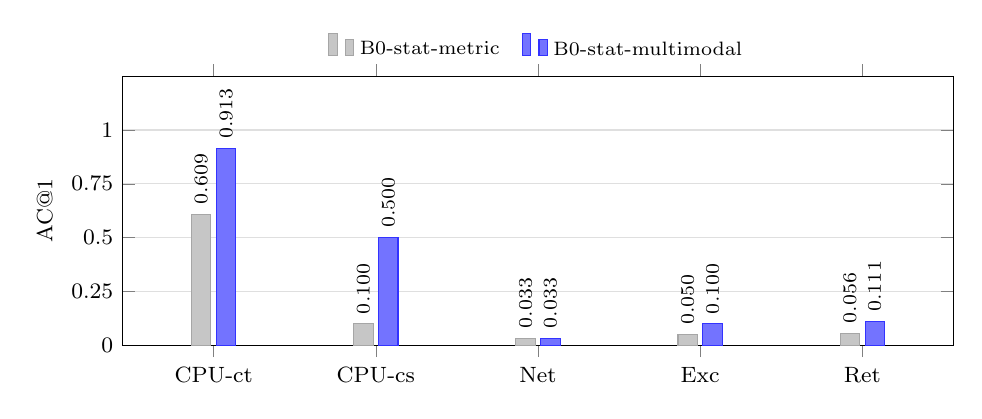
\begin{tikzpicture}
\begin{axis}[
  ybar, bar width=7pt, width=\columnwidth, height=5cm,
  ymin=0, ymax=1.25, ytick={0,0.25,0.5,0.75,1}, ylabel={AC@1}, ylabel style={font=\footnotesize},
  symbolic x coords={CPU-ct,CPU-cs,Net,Exc,Ret},
  xtick=data, tick label style={font=\footnotesize},
  legend style={font=\scriptsize, at={(0.5,1.02)}, anchor=south, draw=none, fill=none, legend columns=2, /tikz/every even column/.append style={column sep=6pt}},
  legend cell align=left,
  nodes near coords={\pgfmathprintnumber[fixed, fixed zerofill, precision=3]{\pgfplotspointmeta}}, every node near coord/.append style={font=\scriptsize, rotate=90, anchor=west},
  enlarge x limits=0.14, ymajorgrids, grid style={gray!25}
]
\addplot[fill=gray!45, draw=gray!70] coordinates {(CPU-ct,0.609) (CPU-cs,0.1) (Net,0.033) (Exc,0.05) (Ret,0.056)};
\addplot[fill=blue!55, draw=blue!80] coordinates {(CPU-ct,0.913) (CPU-cs,0.5) (Net,0.033) (Exc,0.1) (Ret,0.111)};
\legend{B0-stat-metric, B0-stat-multimodal}
\end{axis}
\end{tikzpicture}
\caption{AC@1 by fault type for the two statistical baselines (case counts: CPU-ct 23, CPU-cs 10, Net 30, Exc 20, Ret 18). Fusion helps resource faults but leaves network and code-level faults largely unresolved.}
\label{fig:perfault}
\end{figure}

\subsection{G1: Propagation errors (RQ2)}
B0-stat-multimodal makes 70 top-1 errors. In 25 of them (35.7\%), the top-ranked service is a direct caller or callee of the true root cause (category F1, Table~\ref{tab:failures}), which is the signature of a symptom ranked above its cause. F1 dominates network-delay errors (15 of 29), consistent with delay propagating to adjacent services. H2 is supported: more than one third of errors are, in principle, correctable by a verifier that examines the immediate neighbourhood of the top hypothesis. The verifier itself has not yet been evaluated, so G1 remains open.

\subsection{G2: Cost (RQ3)}
Table~\ref{tab:cost} reports the cost recorded by the harness. Both statistical baselines run in milliseconds per case without model or tool calls. For the LLM-based methods, the scripted provider demonstrates that the harness counts calls for every case: B1 issues exactly one model call, and P0 issues three model calls and five tool calls per case under the configured caps of 8 steps and 20 tool calls. These counts reflect the fixed script, not the behaviour of a real LLM, and the scripted provider reports no token usage. H3 is therefore verified at the pipeline level: investigation is bounded and its cost is accounted for, while the cost--accuracy trade-off for real models remains to be measured.

\begin{table}[t]
\centering
\caption{Mean per-incident cost recorded by the harness. Rows marked $\dagger$ use the scripted provider and validate accounting only.}
\label{tab:cost}
\footnotesize
\setlength{\tabcolsep}{4pt}
\resizebox{\columnwidth}{!}{\begin{tabular}{@{}lrrrr@{}}
\toprule
\textbf{Method} & \textbf{LLM calls} & \textbf{Tool calls} & \textbf{Tokens} & \textbf{Latency (s)} \\
\midrule
B0-stat-metric & 0 & 0 & 0 & 0.028 \\
B0-stat-multimodal & 0 & 0 & 0 & 0.009 \\
B1-single-call$^\dagger$ & 1 & 0 & -- & $<$0.001 \\
P0-react-agent$^\dagger$ & 3 & 5 & -- & 0.028 \\
\bottomrule
\end{tabular}}
\end{table}

\subsection{G3: Memory and RQ4}
The memory protocol is implemented as an interface, but no memory policy has been evaluated, and real-LLM runs of B1 and P0 have not yet been performed. We therefore make no claim about whether the agent improves on B0. As an integration check, the scripted B1 and P0 runs reproduce the AC@1 of B0-stat-metric (0.178) exactly, which is expected because the script answers with the metric-anomaly ranking; it confirms that tool outputs, parsing, and scoring are consistent end to end.

% =====================================================================
\section{Ablation and Comparative Analysis}\label{sec:ablation}

Table~\ref{tab:ablation} isolates the contribution of each fused signal. Removing CPU or memory evidence lowers AC@1 by 0.069 and 0.059, respectively, and removing CPU reduces TT AC@1 from 0.156 to 0.067. Removing server latency or trace latency lowers AC@1 by only 0.010, and removing log evidence slightly \emph{increases} AC@1 to 0.317 while lowering AC@3 and AC@5. A fusion of the three metric signals alone (CPU, memory, server latency) attains AC@1 0.297 and AC@5 0.485, within 0.010 of the full five-signal fusion. Thus, under the current scoring functions, most of the improvement over B0-stat-metric arises from \emph{rank-level fusion of complementary resource metrics}, rather than from logs or traces. This qualifies the conclusion of RQ1: multimodal data are available to the methods, but the log and trace scores used by B0 are too coarse to localize the exception, return, and network faults where they would matter most. This observation motivates on-demand inspection of logs and traces by the agent, rather than fixed aggregate scores.

Single-signal rankings are informative as well. Memory alone yields the highest AC@3 (0.485) and AC@5 (0.594) of any configuration but a lower AC@1 (0.277), indicating that memory deviation is a good candidate filter but a poor discriminator at the top. Log evidence alone is weak (AC@1 0.059), and its TT AC@1 is zero.

\begin{table}[t]
\centering
\caption{Signal ablation of B0-stat-multimodal (RRF over five signals). ``$-$'' removes one signal; ``only'' uses one signal.}
\label{tab:ablation}
\footnotesize
\setlength{\tabcolsep}{3.5pt}
\resizebox{\columnwidth}{!}{\begin{tabular}{@{}lrrrrrr@{}}
\toprule
\textbf{Configuration} & \textbf{AC@1} & \textbf{AC@3} & \textbf{AC@5} & \textbf{Avg@5} & \textbf{OB} & \textbf{TT} \\
\midrule
Full fusion (5 signals) & 0.307 & 0.396 & 0.475 & 0.386 & 0.429 & 0.156 \\
\midrule
$-$ CPU & 0.238 & 0.366 & 0.446 & 0.358 & 0.375 & 0.067 \\
$-$ memory & 0.248 & 0.366 & 0.436 & 0.360 & 0.339 & 0.133 \\
$-$ server p90 latency & 0.297 & 0.416 & 0.475 & 0.398 & 0.411 & 0.156 \\
$-$ trace latency & 0.297 & 0.396 & 0.475 & 0.386 & 0.411 & 0.156 \\
$-$ log & 0.317 & 0.376 & 0.446 & 0.382 & 0.446 & 0.156 \\
\midrule
CPU only & 0.287 & 0.356 & 0.436 & 0.360 & 0.393 & 0.156 \\
memory only & 0.277 & 0.485 & 0.594 & 0.450 & 0.446 & 0.067 \\
server p90 only & 0.178 & 0.337 & 0.455 & 0.321 & 0.304 & 0.022 \\
trace only & 0.218 & 0.327 & 0.465 & 0.341 & 0.321 & 0.089 \\
log only & 0.059 & 0.198 & 0.317 & 0.192 & 0.107 & 0.000 \\
\midrule
Metric signals only (3) & 0.297 & 0.396 & 0.485 & 0.392 & 0.411 & 0.156 \\
\bottomrule
\end{tabular}}
\end{table}

\textbf{Efficiency trade-offs.} The statistical baselines cost no model calls and run in roughly 0.01--0.03\,s per incident, so their accuracy defines the bar that an agent must clear to justify its cost. Each P0 step adds one model call, and the configured caps bound an investigation to at most nine model calls (eight steps plus a forced final answer) and twenty tool calls. Because tool observations are truncated to 4000 characters, the prompt grows by at most a bounded amount per tool call; the actual token cost depends on the model and is recorded by the harness when the provider reports it. B1 represents the lowest-cost LLM configuration, with one call over precomputed summaries, and isolates the value of iterative tool use in P0 from the value of LLM reasoning alone.

\textbf{Comparison with the base paper.}\label{sec:related-compare} OpenRCA grants its agent unrestricted code execution over 68\,GB of telemetry and reports an 11.34\% solve rate for its best configuration~\cite{xu2025openrca}. MicroRCA-Agent instead pre-aggregates telemetry into small bundles and exposes six bounded tools, trading flexibility for auditability and predictable cost. Whether this restricted action space improves accuracy relative to code execution is an empirical question that the planned OpenRCA re-run and the B1/P0 comparison are designed to answer.

% =====================================================================
\section{Failure Analysis}\label{sec:failures}

Table~\ref{tab:failures} gives the frequency of each failure category for B0-stat-multimodal, by system and by fault type.

\begin{table}[t]
\centering
\caption{Outcome categories of B0-stat-multimodal (counts of incidents). F1: top-1 is a direct neighbour of the root cause; F2: root cause in top-5 otherwise; F3: root cause ranked below fifth.}
\label{tab:failures}
\footnotesize
\setlength{\tabcolsep}{4pt}
\resizebox{\columnwidth}{!}{\begin{tabular}{@{}lrrrrr@{}}
\toprule
\textbf{Group} & \textbf{Hit@1} & \textbf{F1} & \textbf{F2} & \textbf{F3} & \textbf{Total} \\
\midrule
Online Boutique & 24 & 13 & 10 & 9 & 56 \\
Train-Ticket & 7 & 12 & 0 & 26 & 45 \\
\midrule
CPU contention & 21 & 2 & 0 & 0 & 23 \\
CPU consumed & 5 & 4 & 1 & 0 & 10 \\
Network delay & 1 & 15 & 6 & 8 & 30 \\
Exception & 2 & 2 & 2 & 14 & 20 \\
Wrong return & 2 & 2 & 1 & 13 & 18 \\
\midrule
\textbf{All} & \textbf{31} & \textbf{25} & \textbf{10} & \textbf{35} & \textbf{101} \\
\bottomrule
\end{tabular}}
\end{table}

\textbf{F3, missed root causes (35 incidents, 50\% of errors).} This is the largest category and is concentrated in code-level faults (27 of the 38 exception and wrong-return cases) and in TT (26 of 45 cases). The median rank of the true root cause is 2 in OB but 20 in TT, where 46 services dilute the signal. Exceptions and wrong return values perturb application behaviour without large resource deviations, so CPU- and memory-dominated fusion ranks them low. A representative case is \texttt{2022-08-22\_04\_00}, a wrong-return fault in OB's \texttt{frontend}, where \texttt{paymentservice} ranks first on a CPU deviation and the true cause ranks seventh.

\textbf{F1, propagation (25 incidents, 36\% of errors).} The top-ranked service is adjacent to the root cause. In \texttt{2022-08-22\_04\_02}, an exception injected into OB's \texttt{frontend} causes its callee \texttt{recommendationservice} to rank first on server p90 latency, while \texttt{frontend} ranks seventh. In \texttt{2022-08-22\_05\_02}, CPU contention in \texttt{currencyservice} is outranked by its caller \texttt{frontend}, with the true cause third.

\textbf{F2, near misses (10 incidents, 14\% of errors).} All occur in OB, where the small service set keeps the root cause within the top five. In \texttt{2022-08-22\_05\_00}, an exception in \texttt{checkoutservice} is ranked second behind \texttt{recommendationservice}.

\textbf{Systematic attractors.} Misranking is not uniformly distributed across services: \texttt{recommendationservice} is the false top-1 in 18 of 32 OB errors, and \texttt{ts-order-service} in 14 of 38 TT errors. Services with naturally volatile latency or high fan-in thus act as attractors for anomaly-based scoring. Two implications follow for the agent: a verifier should test neighbouring services before accepting a hypothesis (F1), and investigation of logs and traces should be directed by the call graph rather than by aggregate anomaly scores (F3).

% =====================================================================
\section{Limitations and Threats to Validity}

\textbf{Internal validity.} The central limitation is that no real-LLM results for B1 or P0 are reported; the scripted provider validates integration only and cannot support any claim about agent quality. The B0 scoring constants (e.g., the 0.3 weight on new log templates, the scale floors) were chosen during development on the same 101 incidents, so mild overfitting cannot be excluded. Services with identical fused scores are ordered by their position in the service list, which can affect AC@$k$ on ties. Latency measurements are wall-clock times on a single machine and vary by a few milliseconds between runs.

\textbf{Construct validity.} AC@$k$ treats the labelled service as the sole root cause; incidents in which several services are legitimately implicated are scored as failures. Fault-type accuracy is conditional on a correct top-1 service and is therefore computed on 18--31 incidents, which makes it unstable. Our failure categories use only one-hop call-graph adjacency and may underestimate multi-hop propagation.

\textbf{External validity.} The evaluation covers 101 incidents from two open-source benchmark systems with injected faults. Real production incidents involve larger topologies, concurrent faults, configuration changes, and noisier telemetry~\cite{zhou2021trainticket,soldani2022survey}. The small per-category counts (as few as 7 cases per fault type in some systems) yield wide confidence intervals, and the TT results show that conclusions drawn on OB do not transfer to larger systems. Results with LLMs will additionally depend on the choice of model, prompt, and provider, and on possible exposure of public benchmark data during model pretraining.

\textbf{Reproducibility.} Preprocessing discards most raw telemetry; methods that require full-resolution logs or traces cannot be evaluated on the bundles without re-running the pipeline.

% =====================================================================
\section{Conclusion}

This paper presented MicroRCA-Agent, a framework that places statistical, single-call, and tool-using agentic RCA methods behind one contract, one tool layer, and one evaluation harness that records both accuracy and cost. On 101 Nezha incidents, rank fusion of multimodal evidence significantly improves top-1 localization over metrics-only scoring (AC@1 0.307 versus 0.178), but an ablation shows that this gain derives mostly from fusing resource metrics, and a failure analysis shows that more than one third of the remaining errors rank a call-graph neighbour of the root cause first, while code-level faults and the larger Train-Ticket system remain largely unresolved. These findings define concrete targets for agentic investigation.

Future work will (i) run B1 and P0 with the same model on all 101 incidents and report accuracy with cost; (ii) implement and evaluate a neighbourhood-checking verifier for G1, an adaptive budget policy for G2, and an incident memory for G3, each through ablation; (iii) re-run OpenRCA's agent under our protocol; and (iv) evaluate on RCAEval as a held-out benchmark~\cite{pham2025rcaeval}.

% =====================================================================
\bibliographystyle{IEEEtran}
\bibliography{references}

\end{document}
